% \chapter{Fungsi (Subprogram)}
\section{Tujuan}
\begin{itemize}[label=$\bullet$, itemsep=-1pt, leftmargin=*]
    % \item Students understand how to create and call functions in C .
    \item Mahasiswa mengerti cara membuat dan memanggil fungsi pada bahasa pemrograman C.
    % \item Students able to pass parameter by value and by reference in C.
    \item Mahasiswa mampu menggunakan passing parameter by value dan by reference pada bahasa pemrograman C.
    % \item Students understand and able to apply recursion in C. 
    \item Mahasiswa mampu mengerti dan mengaplikasikan konsep rekursi pada bahasa pemrograman C.
    
\end{itemize}

\section{Fungsi}
Fungsi adalah sebuah kumpulan statement untuk melakukan tugas spesifik, yang bisa membutuhkan input ataupun tidak, untuk menghasilkan output yang sesuai.
% The advantages of using functions in C programming language are:
Keuntungan menggunakan fungsi pada bahasa pemrograman C adalah:
\begin{itemize}
	% \item Some code snippets can be reusable when using functions. 
    \item Beberapa cuplikan kode dapat digunakan kembali saat menggunakan fungsi.
    % \item We can call C functions any number of times in a program and from any place in a program.
    Kita dapat memanggil fungsi C berapa kali pun dalam suatu program dan dari mana saja dalam suatu program.
    % \item Large C codes can be splitted to several function, thus easier to track.
    \item Program c yang besar dapat dibagi ke dalam beberapa fungsi sehingga dapat dengan mudah untuk dilacak.
\end{itemize}
\subsection{Function Declaration}
% Every C program has atleast one function, that is the main() function. You can also define functions other than main().
Setiap program C mempunyai minimal satu fungsi, yaitu fungsi main(). Anda juga dapat mendefinisikan fungsi selain main()
Syntax :
\begin{verbatim}
    return_type function_name( parameters list){
        // function body
    	return something;
    }
\end{verbatim}
\begin{itemize}
	% \item Return Type.\\ The data type a function has to return.
	\item Return Type.\\ Tipe data yang harus dikembalikan suatu fungsi.
	% \item \verb*|function_name|.\\ The name of the function
    \item \verb*|function_name|.\\ Nama fungsi
	% \item parameters list.\\ 
    % The parameters of the function. 
    \item parameters list.\\ 
    Parameter dari fungsi.
	% \item Function body.\\ The block of code that will be executed when the function is called.
    \item Function body.\\ Kumpulan statemen yang mendefinisikan apa yang dilakukan oleh fungsi.
	% \item \verb|return something;|\\ A statement to return a value (\verb|something|). Returning the function causes the function to end.
    % For functions that doesn't return a value (\verb|void| type function), ending the function can be done by using \verb|return;|
    \item \verb|return something;|\\ merupakan statement untuk mengembalikan nilai dari fungsi. Untuk fungsi yang tidak mengembalikan nilai, dapat digunakan \verb|return_type| \verb|void|. Untuk keluar dari fungsi itu hanya perlu menggunakan statement \verb*|return|
\end{itemize}  

% Example
Contoh

\begin{lstlisting}[language=c]
float TriangleArea(float Base, float Height)
{
	float Area;
	Area = 0.5*Base*Height;
	return Area;
}
\end{lstlisting}


% \subsection{Calling a Function}
\subsection{Memanggil Fungsi} 

\begin{figure}[H]
	\centering
	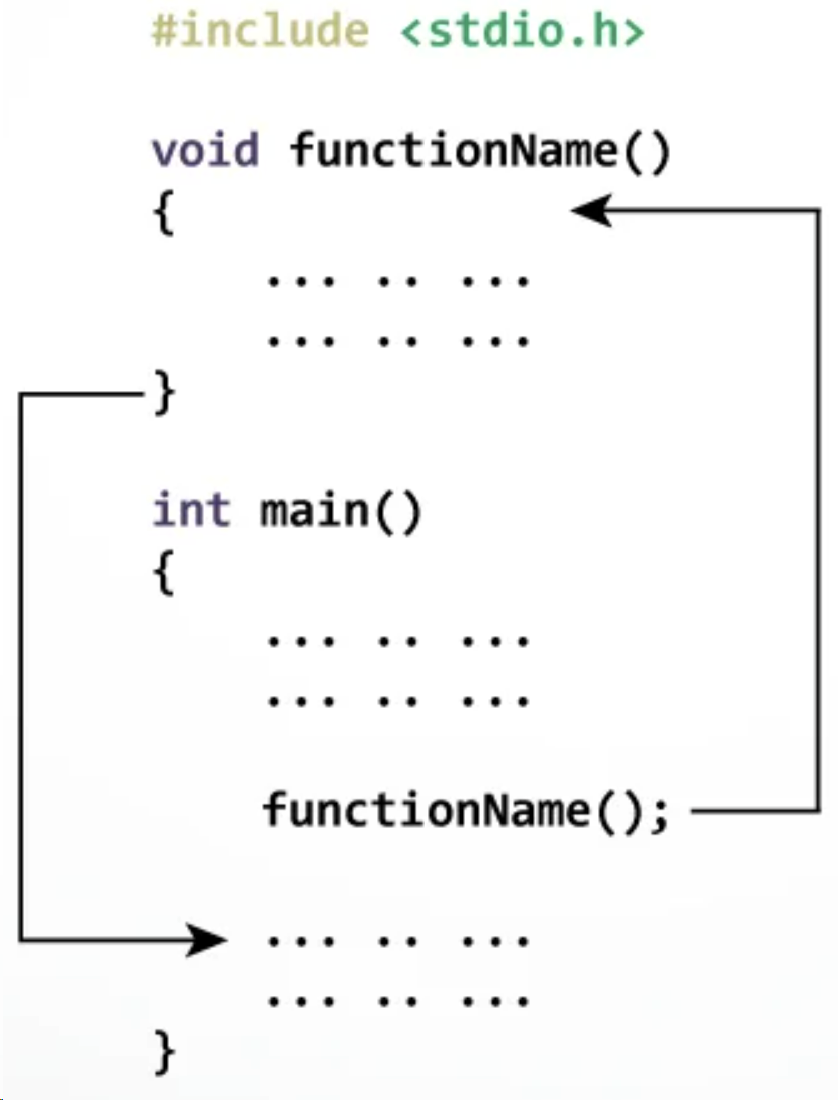
\includegraphics[width=0.45\linewidth]{../P3/img/screenshot005.png}
	\caption{}
	\label{fig:memanggilfungsi}
\end{figure}

\begin{lstlisting}[language=c]
	#include <stdio.h>
// Mendeklarasikan fungsi luasSegitiga
// Parameter input Alas , dan Tinggi
// Output float
float TriangleArea(float Base, float Height)
{
	float Area;
	Area = 0.5*Base*Height;
	return Area;
}
int main()
{
	float Bs = 4,Hg=10,L;
    // Memanggil Fungsi TriangleArea
	L=TriangleArea(Bs,Hg);
	printf("Area = %f",L);
	return 0;
}
\end{lstlisting}
\begin{enumerate}
	% \item Line 5-10: Defining the function \verb|Triangle Area| with 
    \item Baris 5-10:Mendefinisikan fungsi \verb*|TriangleArea| dengan 
	\begin{itemize}
		% \item Two input parameter :\\
        \item 2 paramater input/masukan:
	% input \verb*|Base| and \verb*|Height|  with \verb*|float| data type.
    input \verb*|Base| dan \verb*|Height|  dengan tipe data \verb*|float|.
	    \item Output bernilai tunggal dengan tipe data \verb*|float|.
    \end{itemize}
\end{enumerate}
% \subsection{Function with Arguments}
\subsection{Fungsi dengan Argumen}

\subsubsection{Argumen}


Jika suatu fungsi diharapkan untuk menggunakan argumen, maka variabel sebagai parameter yang menerima nilai dari argumen tersebut harus di dedeklarasikan terlebih dahulu. \\
\begin{enumerate}
	\item  \textbf{Parameter :}
\begin{enumerate}
	\item Parameter adalah variabel dalam fungsi untuk merujuk ke salah satu bagian dari
	data yang diberikan sebagai input ke fungsi.
    % \item Parameters are the variable in the function that points to the part of the data that is inputted to the function.
	\item Data ini disebut argumen.
    % \item These data is called arguments.
	
\end{enumerate}

\item \textbf{Formal Parameter:}
\begin{enumerate}
	\item Parameter yang Ditulis dalam Definisi Fungsi Disebut "Parameter Formal".
    % \item Parameter that is written within the function definition is called formal parameter.
	\item Parameter formal selalu variabel, sedangkan parameter aktual tidak harus variabel.
	% \item Formal Parameter is always a variable, Actual Parameter however doesn't necessarily has to be a variable.
	
\end{enumerate}


\item \textbf{Actual Parameter:}
\begin{enumerate}
	
    % \item Parameter that is used when calling the function
    \item Parameter yang Ditulis ketika memanggil fungsi.
    % \item Actual Parameter could take the form of number, expression, or another function call.
	\item Dapat berupa angka, ekspresi, atau bahkan panggilan fungsi.
\end{enumerate}
\begin{figure}[H]
	\centering
	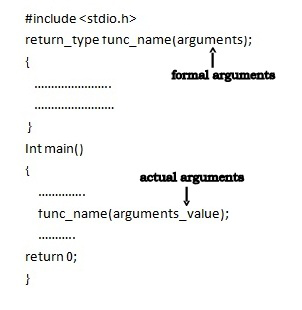
\includegraphics[width=0.5\linewidth]{../P3/img/screenshot006.png}
	\caption{}
	\label{fig:parameterformalaktual}
\end{figure}
\end{enumerate}
\subsection{Parameter Passing} 
Passing parameter merupakan aktivitas menyalurkan nilai pada parameter saat memanggil fungsi. Pada umumnya, dikenal dua macam passing parameter yaitu:
% To use a function with parameter, the parameters must be passed to the function first.
% In general, there are two ways to pass paramater to a function
\begin{itemize}
	% \item Pass parameter by value, pass the value of the variable to the function.
    \item Pass parameter by value, yaitu menyalurkan \textbf{nilai} dari tiap parameter yang diberikan.
	% \item Pass parameter by reference, pass the reference of a variable (its memory address) to the function. 
    \item Pass parameter by reference, yaitu menyalurkan \textbf{alamat} dari tiap parameter yang diberikan.
\end{itemize}

\subsubsection{Passing Parameter by Value}

\begin{lstlisting}[language=c,caption = Passing by Value,label=lst:passbyvalue01]
#include<cstdio>
int swapAndReturnTheSum(int x, int y) {
    int z;
    z = x;
    x = y;
    y = z;
    return x+y;
}
int main()
{
    int a = 1;
    int b = 2;
    int sum = swapAndReturnTheSum(a,b);
    printf("sum: %d\n",sum);
    printf("values of a dan b now:\n");
    printf("a: %d\n",a);
    printf("b: %d\n",b);
}
\end{lstlisting}

Perhatikan potongan kode pada Listing \ref{lst:passbyvalue01}. Baris 3-6 dari kode tersebut adalah operasi untuk menukar nilai dari 2 variabel. Namun, apabila program tersebut dijalankan, maka akan muncul output
% line 3-6 of the code in Listing \ref{lst:passbyvalue01} is a set of assignments to swap the values of 2 variable. However, when the program is executed, the output would be the following.
\begin{verbatim}
    sum: 3
    values a and b now:
    a: 1
    b: 2
\end{verbatim}
% The values of a and b did not swap. When passing parameter by value, anything that is done within the function body will have no effect on the parameter that is "passed on" the function. The value of the actual parameter will be assigned to the formal parameter, so we are not doing operation directly on the actual parameter.
Nilai dari a dan b tidak bertukar. Untuk passing parameter by value, apapun yang dilakukan pada function body tidak akan berpengaruh pada parameter yang "dipassingkan". Nilai dari parameter aktual akan diassign pada parameter formal.

\subsubsection{Passing Parameter by Reference}
Perhatikan baris 2 pada potongan kode berikut:
% Look at line 2 of the following code.
\begin{lstlisting}[language=c,caption = Passing by Reference,label=lst:passbyreference01]
#include<cstdio>
int swapAndReturnTheSum(int &x, int &y) {
    int z;
    z = x;
    x = y;
    y = z;
    return x+y;
}
int main()
{
    int a = 1;
    int b = 2;
    int sum = swapAndReturnTheSum(a,b);
    printf("sum: %d\n",sum);
    printf("values of a dan b now:\n");
    printf("a: %d\n",a);
    printf("b: %d\n",b);
}
\end{lstlisting}
Apabila program tersebut dijalankan, maka akan muncul output
% When this program is executed, it will output the following.
\begin{verbatim}
    sum: 3
    values of a and b now
    a: 2
    b: 1
\end{verbatim}

Ketika fungsi \verb|swapAndReturnTheSum(a,b)| dipanggil, alamat memori variabel a dan b "dipassingkan" pada fungsinya. Sehingga pada pada potongan kode di baris 4-6, x dan y akan mengacu pada memori parameter aktual yang dimasukkan di baris ke 13. Ketika melakukan passing by reference, kita tidak bisa memanggil fungsi dengan parameter yang tidak memiliki alamat memori. Sebagai contoh \verb|tukarDanKembalikansumnya(1,2)| tidak bisa dilakukan karena angka 1 dan 2 bukan variabel dan tidak memiliki alamat memori.
% When the function \verb|swapAndReturnTheSum(a,b)| is called, the memory address of \verb|a| and \verb|b| is passed on to the function. Therefore, in line 4-6, the \verb|x| and \verb|y| will point to the memory of the actual parameter that is inputted in line 13, so we are doing assignments directly to the actual parameter. When passing by reference, we can't call the function with parameter that has no memory address. As example \verb|swapAndReturnTheSum(1,2)| cannot be done as the number 1 and 2 doesn't have memory address.

\subsection{Tugas Pendahuluan}
\begin{enumerate}
   \item Buatlah fungsi yang dapat menerima 2 buah bilangan bulat a dan b kemudian mengembalikan nilai dari $a^b$
    % \item Create a function that can take 2 integer a and b then returns $a^b$
   \item Masalah-masalah apa yang akan lebih mudah diselesaikan dengan menggunakan fungsi?
    % \item What problems that can be solved easier with functions?
\end{enumerate}

\section{Rekursi}
Rekursi merujuk kepada definisi suatu hal yang dilakukan secara berulang-ulang.

Rekursi adalah ketika suatu fungsi dalam function bodynya memanggil fungsi itu sendiri.
% Recursion is when a function calls itself within its function body.
Sebagai contoh, perhatikan potongan kode berikut:
% As an example, look at the code below.
\begin{lstlisting}[language=c,caption = Factorial dengan rekursi,label=lst:recursionexample01]
int factorial(int n) {
    if (n==1)
        return 1;
    return n*factorial(n-1);
}
\end{lstlisting}
The factorial function calls another factorial function in line 4.
%Dapat dilihat bahwa fungsi factorial pada function bodynya memanggil factorial pada baris 4.
Initialy, the function $factorial(n)$ is called. This function however will return 
%Pada awalnya jika fungsi $factorial(n)$ dipanggil maka dia akan mencoba untuk mengembalikan
% $n\times factorial(n-1)$, then $factorial(n-1)$ akan mengembalikan $(n-1)\times factorial(n-1-1)$.
$n\times factorial(n-1)$, kemudian $factorial(n-1)$ akan mengembalikan $(n-1)\times factorial(n-1-1)$.
% Eventually it became like this:
Akhirnya menjadi seperti ini:
\begin{equation*}
    \begin{split}
        factorial(n)& = n \times factorial(n-1)\\
        & = n \times (n-1) \times factorial(n-2)\\
        & = n \times (n-1) \times (n-2) \times \cdots \times 2 \times factorial(1)\\
        & = n \times (n-1) \times (n-2) \times \cdots \times 2 \times 1\\
    \end{split}
\end{equation*}

\subsection{Tugas Pendahuluan}
\begin{enumerate}
   \item Diberikan sebuah baris bilangan 1, 5, 14, 30, ... dst. Buatlah sebuah program yang mengimplementasikan fungsi rekursif untuk menentukan bilangan ke-n dari pola tersebut.
\end{enumerate}